\documentclass[12pt]{article}
\usepackage[english]{babel}
\usepackage[utf8x]{inputenc}
\usepackage[T1]{fontenc}
\usepackage{scribe}
\usepackage{listings}
\usepackage{url} 
\usepackage{placeins}
\usepackage{microtype} 
\usepackage[hyphens]{url}

\Scribe{Akshay, Alan, Lakshya, Virendra}
\Lecturer{Abir De}
\LectureNumber{4}
\LectureDate{11 August 2022}
\LectureTitle{ML Terminology}

\lstset{style=mystyle}

\begin{document}
	\MakeScribeTop

%#############################################################
%#############################################################
%#############################################################
%#############################################################

%Intro
\noindent Over the last two lectures, we reviewed probability and linear algebra. Now, we introduce some basic ML terminology.

\section{An Example: Average Consensus}

This example is in continuation from Lecture 3. We have a graph $G = (V,E)$, where $V=\{1,\ldots,n\}$ is the set of vertices, and $E$ is the set of edges. The degree of node $i$ is given by $d_i$. Define the value $x_i(t)$ to be the {\it opinion} of node $i$ at time $t$. ${x_1(0),\dots,x_n(0)}$ are given. For $t\ge 0$,
\begin{equation} \label{eq:1}
	x_i(t+1) = \frac {\sum_{j\in \mathcal{N}(i)} x_j(t)}{|\mathcal{N}(i)|}
\end{equation}
where $\mathcal{N}(i)$ denotes the set of neighbors of node $i$. That is, the opinion of $i$ at time $t+1$ is average of the opinions of its neighbors at time $t$.
\\

\noindent Consider $\x(t) = [x_1(t) \cdots x_n(t)]^T$. Define $\A \in \mathbb{R}^{n\times n}$ such that $\A\x(t) = \x(t+1)$. From \eqref{eq:1}, $\A$ is a doubly-stochastic matrix, i.e., its entries are non-negative, and its rows and columns add up to $1$. For instance, the first row of $\A$ is of the form $[a_{1j}]^T$, where $a_{1j}=1/d_1$ if $j\in \mathcal{N}(i)$, else $0$. Moreover, ${\bf 1}$ and ${\bf 1}^T$ are right and left eigenvectors of $\A$, with eigenvalue one.
\\

\noindent We state the following result from \cite{averageconsensus}. $\W$ is the weight matrix of a connected graph.
\begin{theorem}
	$\lim_{t \to \infty} \W^t = (1/n){\bf 1}{\bf 1}^T$ if and only if
	\begin{gather}
		{\bf 1}^T\W = {\bf 1}^T, \label{eq:2} \\
		\W{\bf 1} = {\bf 1}, \label{eq:3} \\
		\rho(\W - (1/n){\bf 1}{\bf 1}^T) < 1, \label{eq:4}
	\end{gather}
	where $\rho(\cdot)$ denotes the spectral radius of a matrix, i.e., maximum of the absolute values of its eigenvalues.
\end{theorem}

\noindent For $\A$ as defined earlier, \eqref{eq:2} and \eqref{eq:3} are already satisfied. If \eqref{eq:4} also holds, then for all nodes $i$, $\lim_{t\to \infty} x_i(t) = \frac{\sum_{j=1}^{n} x_j(0)}{n}$.


%\noindent We state the following result from \cite{doublystochastic}. A stochastic matrix $\M$ is called semi-positive if all entries of some power $\M^\alpha$ are positive.
%\begin{theorem}
%	If $\M \in \mathbb{R}^{n\times n}$ is a semi-positive doubly stochastic matrix, then $\lim_{t\to \infty} \M^t = \frac{1}{n}\J$, where $\J \in \mathbb{R}^{n\times n}$ with all entries $1$.
%\end{theorem}
%
%
%\noindent Thus, if $\A$ is semi-positive and doubly stochastic, then for all nodes $i$, $\lim_{t\to \infty} x_i(t) = \frac{\sum_{j=1}^{n} x_j(0)}{n}$.
%\\
%
%\noindent Some points to note:
%\begin{itemize}
%	\itemsep0em
%	\item $\A$ is symmetric
%	\item $\A{\bf 1} = {\bf 1}$
%	\item ${\bf 1^T}\A = {\bf 1^T}$
%\end{itemize}


\section{Image Classification Problem}


We are given a set of images $\{I_1, \dots, I_n\}$, each corresponding to exactly one of three animal classes: cat, dog, or tiger. The pixel data of $I_i$ is encoded into feature-matrix $X_i \in \mathbb{R}^{d\times d}$, and IDs of the three classes are $\{0,1,2\}$ respectively. \textit{Binary} classification problems involve only two labels, usually $\{0,1\}$.
\\
\begin{figure}[h]

\centering
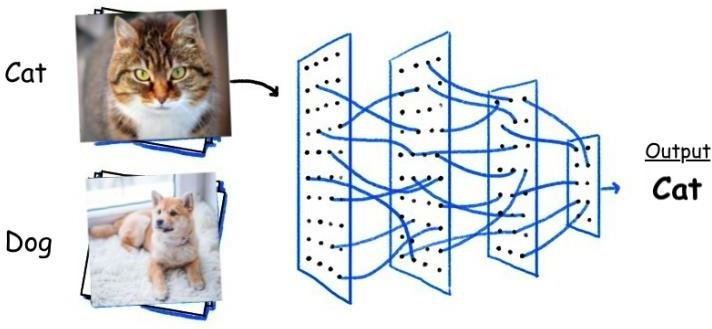
\includegraphics[scale=0.5]{classification.png}
\caption{Dog or Cat? A binary classification example^\cite{binaryclassification}}
\end{figure}


\noindent The goal is to correctly predict the label of any (unseen) image. Unseen images are inputs that were not revealed during the algorithm's development. We can't possibly write an algorithm for this prediction, since the model itself changes with the input space. Moreover, an algorithm with one-to-one mappings for the given set $\{X_i\}$ will perform poorly on unseen images. This is because the model has completely overfit to these images.
\\

\noindent Our approach is to write a program that can design an algorithm for classifying $X_i$s. But this program does not know what the labels represent, or how to differentiate $X_i$s. The problem with just the set of $X_i$'s is ill-defined. Therefore we need to teach this program using some data, which consists of a set of examples $\{X_i\}$, already mapped to corresponding $y_i$s. This brings up the idea of a training set.

\section{Training and Validation Sets}


\subsection{Training Set}
For the classification problem, the training set consists of pairs $(X_i,y_i)$. For each image matrix $X_i$, a label $y_i$ has already been provided, and this label is assumed to be correct. Assuming binary classification, we need to find a function $H : \mathbb{R}^{d\times d} \to \{0,1\}$, such that $H(X_i)=y_i$. As mentioned above, this function should give correct results for unseen images too.
\\

\noindent For finding the {\it best} function from the space of functions, we introduce an error function $L$. Intuitively, $L(f)$ must be large for a function that does the classification job poorly. Then, $H = arg\,min_f L(f)$.

\subsection{Validation Set}
How do we know that the algorithm is ``ready'' for use? Relying only on training set performance isn't a good idea, since the model would have overfit on this data. Thus, we reserve a section of the training data as the validation set. After training the model (on the train set alone), its performance is evaluated on the validation set. Since the latter is unseen during training, we get a more reliable estimate of the model's performance.


\section{(Bonus) Model Selection and the Three-Way Split}
\noindent
In practice, we often train a variety of different models on the same data. This is possible because we have several choices for the architecture of the model and every architecture in turn has several \textit{parameters} we can tune to improve the accuracy. Ideally we'd like to measure the performance of each of these models and choose the one that performs the best on unseen data. 
\\

\noindent That is, we first train the model on one set, then choose the model which performs best on the second set and, once we are done finalizing the model, we use a third set see how well our model generalizes on new data. The second set is called the \textbf{validation set}. The third set, which, in principle, shouldn't be touched until we are done with the complete training of the model, is known as the \textbf{test set}. 
\\
\begin{figure}[h]

\centering
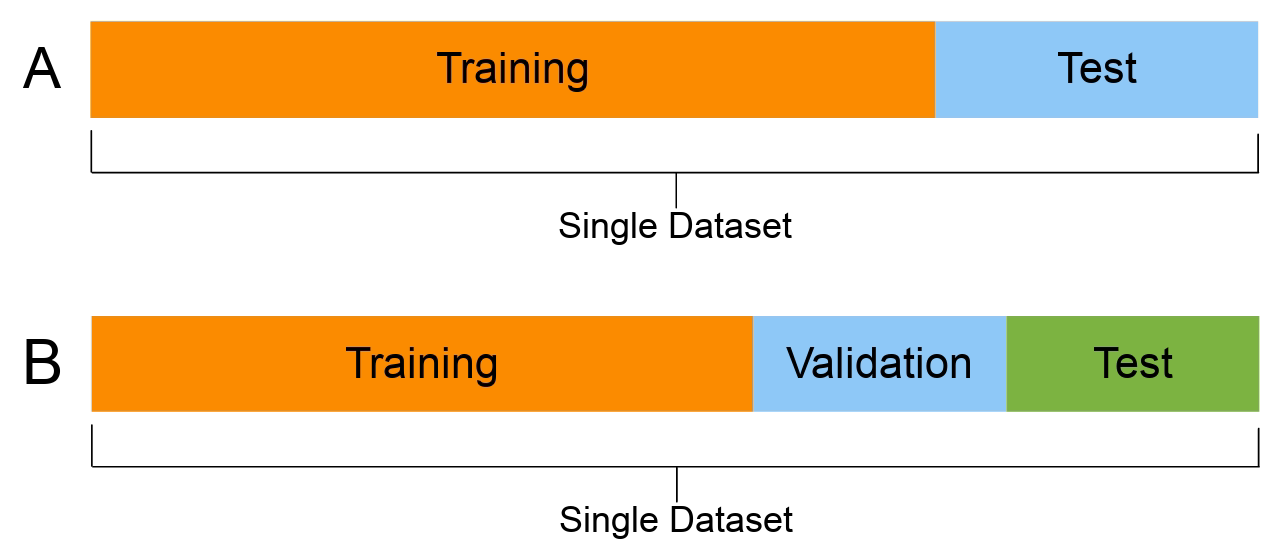
\includegraphics[scale=0.3]{validation.png}
\caption{Three-Way Split into Training, Validation and Test Sets^\cite{twowaysplit}}
\end{figure}


\noindent The fact that we were chose our model based on the second set implies that our model is \textit{learning} the second set. This motivates the need for a third set, without which we'd never know how well our final model generalizes on unseen data because it has already ''seen'' the validation set. 
\\

\noindent We talked about training, validation and test sets. But sometimes, we don't have enough data to justify a three-way split. It is in these cases that we employ a technique known as \textbf{cross-validation}.  \cite{crossvalidation} is a great place to read more about it.


\begin{figure}[h]

\centering
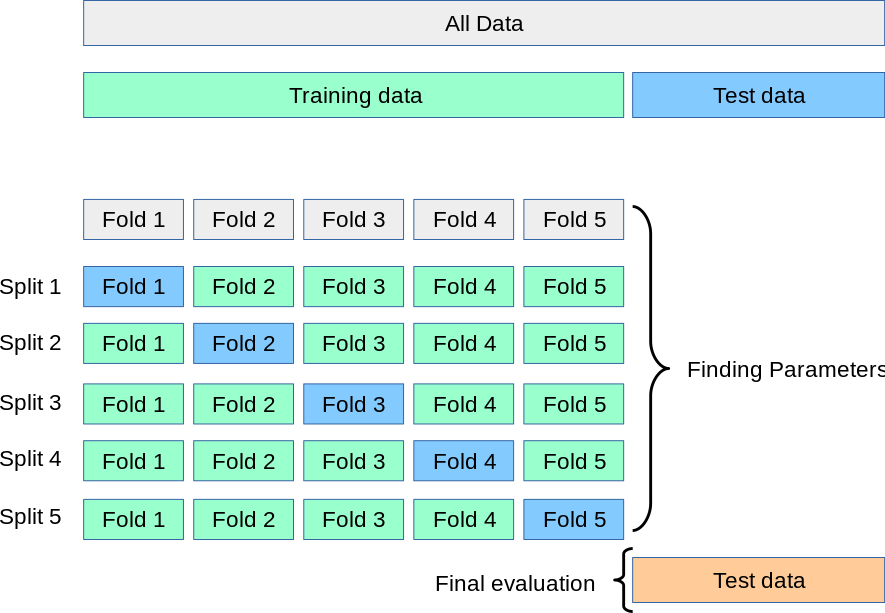
\includegraphics[scale=0.5]{crossvalidation.png}
\caption{Cross-Validation^\cite{crossvalidation}}
\end{figure}


\FloatBarrier



%%%%%%%%%%% If you don't have citations then comment the lines below:
%

{\raggedright % <================================== only left justified!
\bibliographystyle{abbrv}           % if you need a bibliography
\bibliography{mybib}                % assuming yours is named mybib.bib
} % <============================================== ends left justifing!



%%%%%%%%%%% end of doc
\end{document}
